\documentclass[main.tex]{subfiles}
\begin{document}

\chapter{Neutron Stars}

\section{Magneto-rotational evolution}

\subsection{Basic parameters}

\marginpar{Tuesday\\ 2020-11-24, \\ compiled \\ \today}

Their radius is of the order of \SI{10}{km}, their masses are of the order of \(M_{\odot} \sim \SI{2e33}{g}\). 

They rotate very fast, and they are highly magnetized. 
These two facts are quite natural, as can be shown by a back-of-the envelope calculation: angular momentum is conserved, so \(I_* \omega _* = I_{NS } \omega _{NS}\), so considering a Sun-like star we have initially \(R_* \sim \SI{e11}{cm}\); \(P_* \sim \SI{10}{d}\). 

The moment of inertia is \((2/5) M R^2\), so if the star collapses down to NS dimensions while conserving angular momentum we must have
%
\begin{align}
M_* R_*^2 \omega _* = M_{NS} R_{NS}^2 \omega _{NS}
\,,
\end{align}
%
so assuming that the mass is also conserved in the collapse we find 
%
\begin{align}
\frac{R_{NS}^2}{P_{NS}} =
\frac{R_{*}^2}{P_*}
\,,
\end{align}
%
which means 
%
\begin{align}
P_{NS} \sim \underbrace{\qty(\frac{\SI{e6}{cm}}{\SI{e11}{cm}})^2}_{\num{e-10}} \SI{e6}{s} = \SI{e-4}{s}
\,.
\end{align}

This is indeed quite unrealistic, but it shows the point quite well. 
However, these stars cannot rotate too much: the \textbf{mass shedding limit} is reached when the centrifugal force on the material on the surface equals the gravitational pull, so in a Newtonian fashion
%
\begin{align}
\frac{GM}{R^2} = R \omega^2 \implies \nu = \SI{1836}{Hz}  \qty(\frac{M}{M_{\odot}})^{1/2}  \qty( \frac{R}{\SI{e6}{cm}})^{-3/2}  
\,,
\end{align}
%
and millisecond pulsars have been observed.

Regarding magnetism, because of flux conservation \(B_* R_*^2 = B_{NS} R_{NS}^2\). How large is \(B_*\) for a typical star?
This has a large variability, but typically it is of the order of \SI{100}{G}. 
This yields 
%
\begin{align}
B_{NS} = B_* \qty(\frac{R_*}{R_{NS}})^2 \sim \SI{e12}{G}
\,.
\end{align}

These fields get close to \(B_{QED} = \SI{4.4e13}{G}\), at which point quantum relativistic effects start to become relevant, since the cyclotron frequencies of electrons, \(\omega _c = q B / m_e c\), are such that the energies of the quantized cyclotron orbits are comparable to \(m_e c^2\).\footnote{The threshold is, in SI units, calculated as 
%
\begin{align}
B _{\text{QED}} = \frac{(m_ec)^2}{e \hbar}
\,.
\end{align}
}

What we will study will be the magneto-rotational evolution of the NS. 
What is the topology of the \(\vec{B}\) field? We \textbf{do not know}. 
The magnetic field is ``frozen'' as the star rotates; we will start out by the first-order contribution: the dipole. A sketch is shown in figure \ref{fig:dipole-field}

\begin{figure}[ht]
\centering
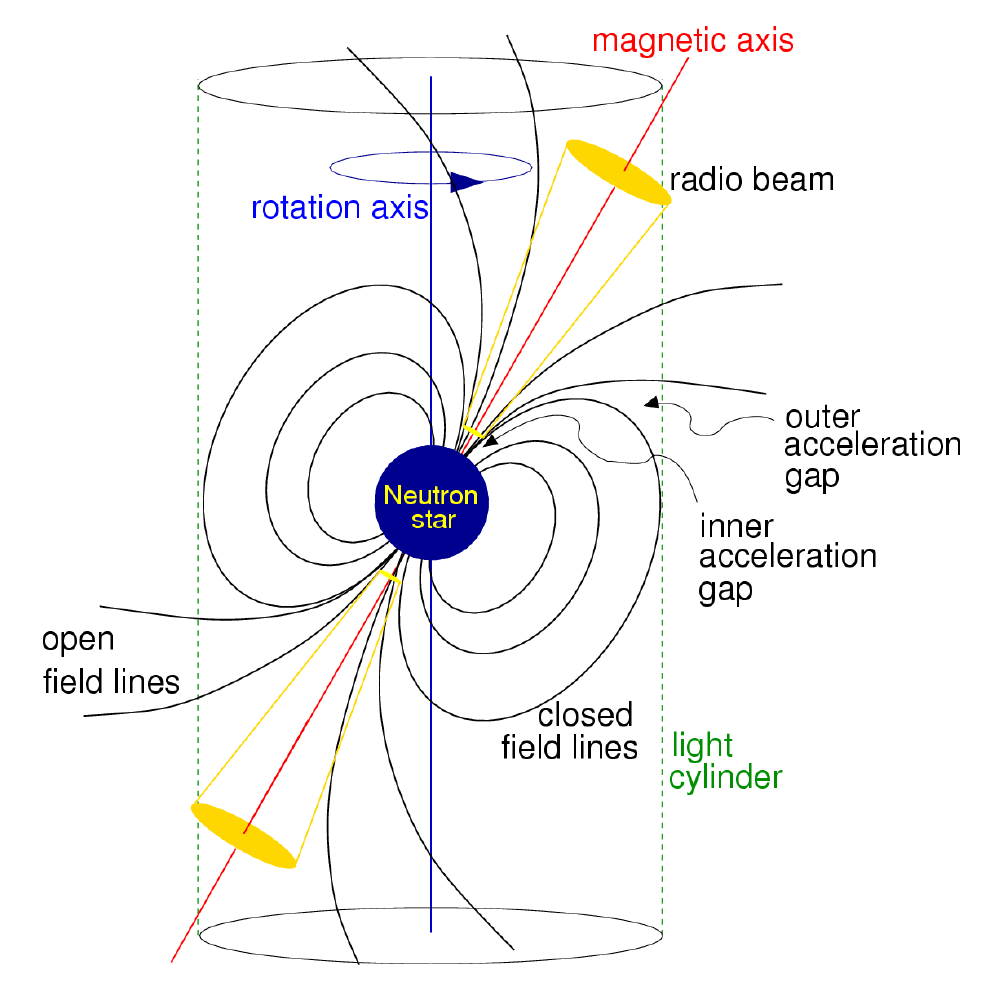
\includegraphics[width=.8\textwidth]{figures/dipole-field.png}
\caption{Dipolar magnetic field of a Neutron Star.}
\label{fig:dipole-field}
\end{figure}

This is given by 
%
\begin{align}
\vec{B} _{\text{dip}} = \underbrace{\frac{B_p}{2} \qty( \frac{R_{NS}}{R})^3}_{= \abs{\vec{m}} / 2R^3}
\times \qty(2 \cos \theta \hat{u}_r + \sin \theta \hat{u}_\theta )
\,,
\end{align}
%
where \(B_p\) is the polar magnetic field. 
The magnetic moment has magnitude \(m = B_p R_{NS}^3\). 

We can decompose it in cartesian coordinates: \(\vec{m} = (m_x, m_y, m_z)\); and similarly in polar coordinates: \(\alpha \) (the angle between \(\vec{m}\), the magnetic axis, and \(\vec{\Omega}\), the rotation axis) and \(\psi = \Omega t\) (the azimuthal angle, rotating around \(\vec{\Omega}\)). 

The rotation is much faster than the evolution of the interior structure, so we will have 
%
\begin{align}
\dot{\vec{m}} &= m \qty(- \Omega \sin \alpha \sin \Omega t, \Omega \sin \alpha \cos \Omega t , 0)  \\
\ddot{\vec{m}} &= m \Omega^2 \sin \alpha \qty(\cos \Omega t, - \sin \Omega t, 0) 
\,,
\end{align}
%
therefore the modulus is \(\ddot{m} = m \Omega^2 \sin \alpha \). 
The \textbf{Larmor formula} for the power lost per unit time gives us 
%
\begin{align}
P = \frac{2 \ddot{m}^2}{3 c^3} = \frac{2}{3 c^3} m^2 \Omega^{4} \sin^2 \alpha 
\,.
\end{align}

Where does this energy come from? The star could even be at zero temperature and still emit, the rotational energy \(E_K = I \Omega^2 /2\) is instead the reservoir. 
The order of magnitude for the moment of inertia is roughly \(I = 2 M R^2 /5 \sim \SI{e45}{g cm^2}\). 

The variation of rotational energy will be 
%
\begin{align}
\dot{E}_K = I \Omega \dot{\Omega} = - P 
\,,
\end{align}
%
therefore 
%
\begin{align}
I \Omega \dot{\Omega} &= - \frac{2}{3c^3} B_p^2R_{NS}^{6} \Omega^{4} \sin^2\alpha   \\
\dot{\Omega} &= - \underbrace{\frac{2}{3 I c^3} B_p^2R_{NS}^{6} \sin^2\alpha}_{A} \Omega^{3} 
\,,
\end{align}
%
which tells us that there will be a secular decrease in the rotation rate of the neutron star. This is immediately integrated: 
%
\begin{align}
\frac{\dot{\Omega}}{\Omega^3} = - A \implies
\frac{1}{2 \Omega_0^2} = \frac{1}{2 \Omega^2} - A(t - t_0 ) 
\,.
\end{align}

A useful approximation is \(\Omega_0 \gg \Omega \), meaning that the NS is quite old --- this is the case very quickly immediately for NSs with periods of the order of \SI{1}{s}. 
This means that we can neglect \(\Omega_0^{-2}\), therefore 
%
\begin{align}
\Omega^{-2} \approx 2 A t
\,,
\end{align}
%
which means \(\Omega \propto t^{-1/2}\). 
This is known as the spin-down. 
The period is 
%
\begin{align}
P^2 = \frac{4 \pi^2}{\Omega^2}
= \frac{16 \pi^2}{3 c^3 I} B_P^2 R_{NS}^{6} \sin^2 \alpha  \times t
\,.
\end{align}

We can also write 
%
\begin{align}
\frac{ \dd{P}}{P} = - \frac{\dd{\Omega}}{\Omega }
\,,
\end{align}
%
therefore 
%
\begin{align}
P \dot{P} = -(4 \pi)^2 \frac{\dot{\Omega}}{\Omega^3}
= \frac{8 \pi^2 B_P^2 R_{NS}^{6} \sin^2\alpha }{3 I c^3} 
\,.
\end{align}

In other words, 
%
\begin{align}
B_P = \sqrt{P \dot{P}} \sqrt{\frac{3 I c^2}{8 \pi^2 R_{NS}^{6} \sin^2 \alpha }}^{1/2}
\approx \frac{\SI{6e19}{G}}{\sin \alpha } \sqrt{ \frac{P\dot{P}}{\SI{1}{s}} }
\,.
\end{align}

This allows us to directly measure \(B_P\), as long as we have some good estimates for \(R_{NS}\) and \(I\). Typically, \(P \sim \SI{1}{s}\) and \(\dot{P} \sim \SI{e-14}{s/s}\). 
This yields \(B_P \sim \SI{e12}{G}\). 

The age of the NS can be estimated as \(t \approx P / 2 \dot{P}\); which is typically found to be of the order of \SI{e5}{yr}.

\end{document}
